%% Fall 2013 MDM Homework Template
\documentclass[12pt,letterpaper]{article}

\usepackage[utf8]{inputenc}
\usepackage[T1]{fontenc}
\usepackage{amsmath}
\usepackage{amsfonts}
\usepackage{amssymb}
\usepackage[left=2cm,right=2cm,top=2cm,bottom=2cm,headheight=22pt]{geometry}
\usepackage{fancyhdr}
\usepackage{setspace}
\usepackage{lastpage}
\usepackage{graphicx}

\begin{document}

%other parameters
\setlength{\parskip}{1ex plus 0.5ex minus 0.2ex}
\setlength{\parindent}{0pt}

%header and footer parameters
\pagestyle{fancy}
\lhead{Math 1100}
\chead{Weekly Homework}
\rhead{Due: February 6}
\lfoot{}
\cfoot{\emph{Prof. Hitchman}}
\rfoot{}

\begin{center}
{
\Large
\textbf{Written Assignment \#3}
}
\end{center}

We have seen the following knot before, and noted that it is a planar projection of an unknot.
Show that this knot is equivalent to the unknot be describing a sequence of Reidemeister moves which change this planar projection into an ordinary circle.
Draw pictures of the steps along the way, and clearly label each transition with the type of move made.

\vspace{1cm}



\begin{figure}[h]
    \centering
    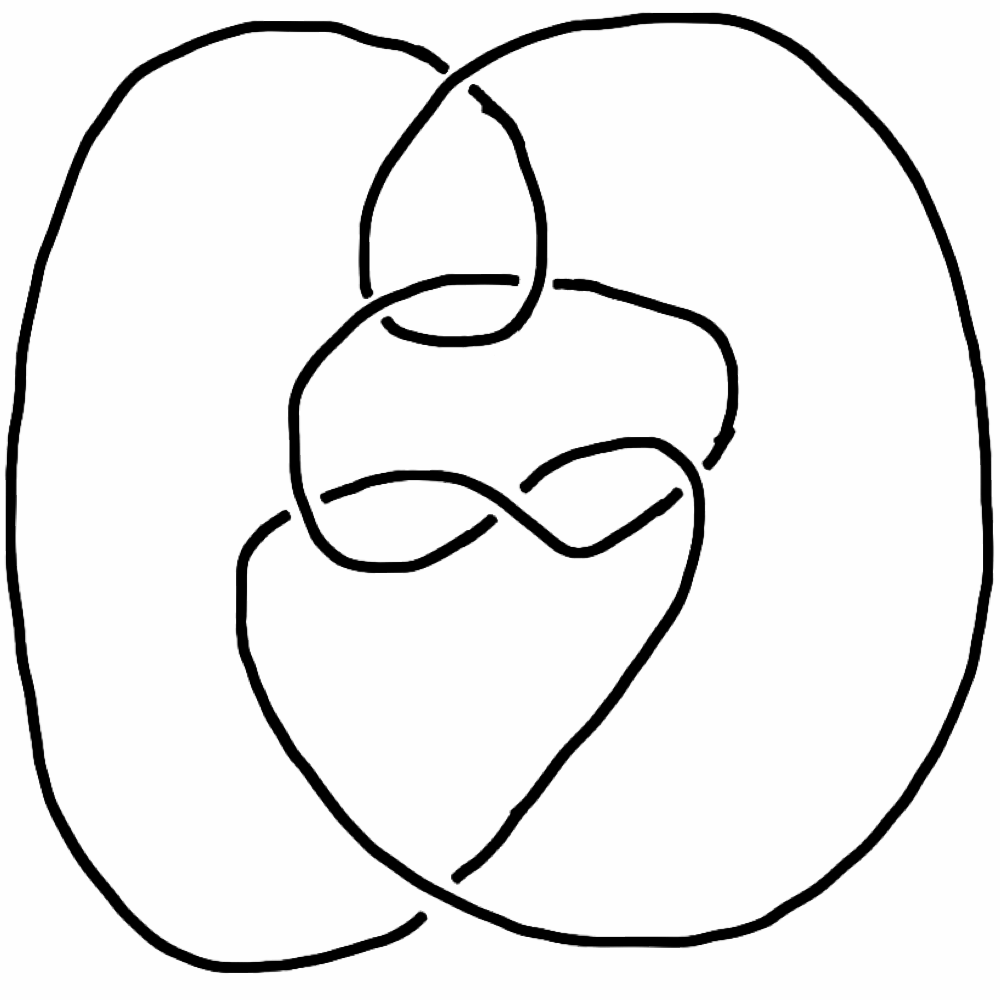
\includegraphics[width=.7\textwidth]{knotpics/9SeptQ5b.png}
    \caption{An Unknot}
\end{figure}

To earn a passing mark, your assignment must:
\begin{itemize}
\item be written legibly. Diagrams may be hand drawn, but should be clear enough to read easily.
\item address the writing prompt above.
\item conform to reasonable standards for grammar, spelling, and usage of the English language with minimal errors. (You may consider seeking help on writing from the Writing Center in the Academic Learning Center. http://www.uni.edu/unialc/writing-center)
\item be turned in by 2pm (the end of class) on Friday, February 6.
\end{itemize}


\end{document}
%sagemathcloud={"zoom_width":100}